% =====================================================================
%  Guaranteed equilibrated a posteriori error estimation for
%  phase-field fracture via Hu--Zhang stress, with stress-driven
%  adaptivity.
%
%  DRAFT (2026-06-21). 计算数学定位；正文不写软件/库/版本（见仓库写作规范）。
%  理论细节见 docs/adaptive/THEORY_equilibrated_aposteriori.md (Thm 1/2)、
%  THEORY_marking_strategy.md (M-DF)、DECISION_sigma_driven_adaptivity.md；
%  数值见 docs/adaptive/RESULTS_aposteriori.md。
% =====================================================================
\documentclass[11pt]{article}
\usepackage[margin=1in]{geometry}
\usepackage{amsmath,amssymb,amsthm,bm}
\usepackage{graphicx}
\usepackage{booktabs}
\usepackage{hyperref}

\newtheorem{theorem}{Theorem}
\newtheorem{proposition}{Proposition}
\newtheorem{assumption}{Assumption}
\newtheorem{remark}{Remark}

\newcommand{\Om}{\Omega}
\newcommand{\eps}{\varepsilon}
\newcommand{\dv}{\operatorname{div}}
\newcommand{\CC}{\mathbb{C}}
\newcommand{\Cd}{\mathbb{C}_d}
\newcommand{\Ad}{\mathbb{A}(d)}
\newcommand{\Sig}{\mathbb{S}}
\newcommand{\Hdiv}{H(\dv;\Sig)}
\newcommand{\GN}{\Gamma_N}
\newcommand{\GD}{\Gamma_D}
\newcommand{\kres}{k_{\mathrm{res}}}
\newcommand{\osc}{\mathrm{osc}}
\graphicspath{{../../figures/adaptive/}}

\title{Guaranteed equilibrated a posteriori error estimation for
phase-field brittle fracture via Hu--Zhang stress,\\
with stress-driven mesh adaptivity}
\author{(authors)}
\date{Draft \today}

\begin{document}
\maketitle

\begin{abstract}
We propose a guaranteed, constant-free a posteriori error estimator for the
elastic sub-problem of staggered phase-field brittle fracture. The key
observation is that a symmetric, $H(\dv)$-conforming mixed (Hu--Zhang)
discretization delivers a \emph{pointwise equilibrated} stress at no
reconstruction cost: it is a member of the statically admissible set, exactly
what the Prager--Synge hypercircle identity requires for the stress side.
Pairing this stress with a standard conforming displacement yields a
reliability constant of exactly one; for the canonical fracture setting
(vanishing body force, traction-free crack faces, displacement loading) the
bound carries \emph{no data oscillation}. We analyse the effectivity under the
degraded coefficient $\Cd=g(d)\CC$ and show, both theoretically and
numerically, that the effectivity index follows the \emph{local} coefficient
contrast on a patch -- which stays $O(1)$ because the phase field is smooth at
the patch scale -- rather than the global residual stiffness $\kres^{-1}$. The
same equilibrated stress drives a predictive, stress-based marking strategy
(M-DF) within a predictor--corrector adaptive loop. Numerical experiments on
single-edge tension and shear confirm reliability and an effectivity index
converging to $1^+$ ($\eta$ exceeds the true error by $4.4\%$), and demonstrate
that adaptivity attains the reference peak load to within $1.5\%$ using
$93\%$ fewer stress degrees of freedom than a uniform mesh of matching accuracy.
\end{abstract}

\section{Introduction}
Phase-field models regularize brittle fracture by a damage field
$d\in[0,1]$ that degrades the elastic energy through $g(d)=(1-d)^2+\kres$. The
displacement sub-problem is solved on a mesh that must resolve the regularization
length $\ell_0$ inside the crack band; under-resolution ($h/\ell_0\gtrsim1$)
systematically \emph{overestimates} the peak load. Reliable, local error control
is therefore essential, yet the classical guaranteed estimators of equilibrated
type require a stress field in the statically admissible set $\Sigma_f$ --
something a standard conforming displacement discretization does not provide and
must \emph{reconstruct} (e.g.\ by Braess--Sch\"oberl local problems).

Our thesis is that the cost of a symmetric $H(\dv)$-conforming mixed stress
element (Hu--Zhang) is repaid precisely here: it produces an equilibrated stress
\emph{directly}, making the hypercircle bound available without reconstruction
and with reliability constant one. We develop the estimator
(Section~\ref{sec:est}), analyse its effectivity under degradation
(Section~\ref{sec:eff}), use the same stress to drive predictive adaptivity
(Section~\ref{sec:adapt}), and validate the whole chain numerically
(Section~\ref{sec:num}).

\section{Model problem and equilibrated stress}\label{sec:model}
Let $\Om\subset\mathbb R^2$ with $\partial\Om=\GD\cup\GN$. Within a staggered
step the damage $d$ is frozen, and the displacement solves, with
$\Cd:=g(d)\CC$ and $\Ad:=\Cd^{-1}=g(d)^{-1}\CC^{-1}$,
\begin{equation}
-\dv\!\big(\Cd\,\eps(u)\big)=f \text{ in }\Om,\quad
u=u_D \text{ on }\GD,\quad \Cd\eps(u)\,n=t_N \text{ on }\GN.
\label{eq:strong}
\end{equation}
We require $g\ge\kres>0$ (the weighted norms below degenerate otherwise). Define
the energy and complementary norms
$\|\eps\|_{\Cd}^2=\int_\Om g\,\eps:\CC\eps$ and
$\|\tau\|_{\Ad}^2=\int_\Om g^{-1}\tau:\CC^{-1}\tau$, the kinematically
admissible set $V_g=\{v\in H^1(\Om)^2: v=u_D\text{ on }\GD\}$, and the
statically admissible set
$\Sigma_f=\{\tau\in\Hdiv: -\dv\tau=f,\ \tau n=t_N\text{ on }\GN\}$.

\paragraph{Hu--Zhang stress is a member of $\Sigma_f$.}
The mixed element gives a stress $\sigma_h$ that is (i) pointwise symmetric,
(ii) $H(\dv)$-conforming, and (iii) discretely equilibrated against a
\emph{discontinuous} displacement test space, whence
$\dv\sigma_h=-P_hf$ elementwise ($P_h$ the $L^2$ projection) and
$\sigma_h n=\Pi_h t_N$ on $\GN$. Hence $\sigma_h\in\Sigma_f$ \emph{exactly}
iff $P_hf=f$ and $\Pi_ht_N=t_N$. The canonical fracture benchmark
($f=0$, traction-free $\GN$, Dirichlet loading) satisfies both exactly, so
$\sigma_h\in\Sigma_f$ with no data oscillation. A standard conforming
displacement stress $\Cd\eps(u_h)$ is normal-discontinuous and not in $\Hdiv$:
this is exactly what makes the equilibrated route unavailable to it.

\section{Equilibrated a posteriori estimator}\label{sec:est}
\begin{theorem}[Prager--Synge / hypercircle]\label{thm:ps}
Let $(u,\sigma)$ solve \eqref{eq:strong} with $\sigma=\Cd\eps(u)$. For any
$v\in V_g$ and any $\tau\in\Sigma_f$,
\begin{equation}
\|\Cd\eps(v)-\sigma\|_{\Ad}^2+\|\tau-\sigma\|_{\Ad}^2
=\|\Cd\eps(v)-\tau\|_{\Ad}^2 .
\end{equation}
Dropping the second nonnegative term,
\begin{equation}
\|\eps(v)-\eps(u)\|_{\Cd}\ \le\ \eta(v,\tau):=\|\Cd\eps(v)-\tau\|_{\Ad},
\label{eq:reliab}
\end{equation}
where the right-hand side is fully computable (no unknown constant).
\end{theorem}
The proof reduces the cross term $\int_\Om\eps(v-u):(\sigma-\tau)$ to a boundary
pairing via integration by parts; it vanishes because $\dv(\sigma-\tau)=0$ in
$\Om$, $v-u=0$ on $\GD$, and $(\sigma-\tau)n=0$ on $\GN$ (details in the
supplementary theory notes). Taking $v=u_h$ (conforming displacement) and
$\tau=\sigma_h$ (Hu--Zhang) gives the computable indicator
\begin{equation}
\eta=\Big(\int_\Om g^{-1}(\Cd\eps(u_h)-\sigma_h):\CC^{-1}(\Cd\eps(u_h)-\sigma_h)\Big)^{1/2},
\qquad \eta^2=\sum_T\eta_T^2,
\label{eq:eta}
\end{equation}
with reliability constant $1$. When $\sigma_h\notin\Sigma_f$, two computable,
higher-order data-oscillation terms appear,
$\|\eps(u_h)-\eps(u)\|_{\Cd}\le\eta+\osc(f)+\osc(t_N)$; both vanish in the
canonical benchmark. (A convex-duality majorant extends the bound to the
tension--compression split; see Section~\ref{sec:eff} and the theory notes.)

\section{Effectivity under degradation}\label{sec:eff}
With $\Theta:=\eta/\|\eps(u_h)-\eps(u)\|_{\Cd}\ge1$, the identity gives
\begin{equation}
\Theta^2=1+\frac{\|\sigma_h-\sigma\|_{\Ad}^2}{\|\Cd\eps(u_h)-\sigma\|_{\Ad}^2}.
\label{eq:theta}
\end{equation}
A naive global bound $\Theta^2-1\le\kres^{-1}(\cdots)$ would blow up as
$\kres\to0$; this is pessimistic. The operative local-efficiency constant
depends on the \emph{patch contrast}
$\kappa_{\omega_T}=\sup_{\omega_T}g/\inf_{\omega_T}g$, which stays $O(1)$
because $d$ is solved from a (smooth) phase-field equation and does not vary
sharply within an element. Thus the effectivity decouples from the global
$\kres$. This is the central claim to be confirmed numerically.

\section{Stress-driven adaptivity}\label{sec:adapt}
The same equilibrated $\sigma_h$ drives a \emph{predictive} marking. Define the
dimensionless crack driving force per element
$\mathcal D_\tau=(2\ell_0/G_c)\max_{q\in T}\mathcal H_{\tau,q}$, with the
softening threshold $\mathcal D_c=1/3$ (AT2 calibration). Marking by
$\mathcal D_\tau\ge\beta\mathcal D_c$ with a size floor $h_T\le\ell_0/c_h$
\emph{leads} damage-based / recovery markers: at initiation $d\equiv0$, so all
$d$-based markers are silent, while the driving force already flags the tip.
Using $\sigma_h$ (order $h^{p+1}$) rather than the displacement stress narrows
mismatch in the marked band. Refinement is applied inside a
predictor--corrector loop (repeated within a load step until the marked set is
empty or the size floor is reached), which removes the peak-load overestimation
of a once-per-step scheme. The equilibrated $\eta$ then certifies the accepted
mesh through one conforming displacement re-solve.

\section{Numerical experiments}\label{sec:num}
Unless stated otherwise: unit square, $\ell_0=0.015$, $\kres=10^{-6}$,
Hu--Zhang stress of degree $3$, conforming displacement for certification.

\paragraph{Effectivity decouples from $\kres$.}
On a manufactured degraded problem with a frozen smooth damage band, sweeping
$\kres\in\{10^{-2},\dots,10^{-7}\}$ leaves the sensitivity ratio
$\sqrt{\Theta^2-1}$ essentially flat (growth $1.09\times$ across five decades,
versus a naive prediction of $\sim\!316\times$), and reliability holds to
machine precision ($\eta/\mathrm{err}=1.000$). This confirms the local-contrast
analysis of Section~\ref{sec:eff}.

\paragraph{Reliability and a tight effectivity on a real crack.}
On the single-edge pre-cracked tension specimen at near-peak load, we measure
the true energy error against a nested uniformly refined reference. The
equilibrated stress satisfies discrete equilibrium and traction-free conditions
to machine precision ($\le3\times10^{-16}$), so $\eta$ is a guaranteed upper
bound. The error converges and the effectivity decreases monotonically to
$\Theta=1.044$ at the finest reference level -- $\eta$ exceeds the true error by
only $4.4\%$ (Figure~\ref{fig:theta}).
\begin{figure}[t]\centering
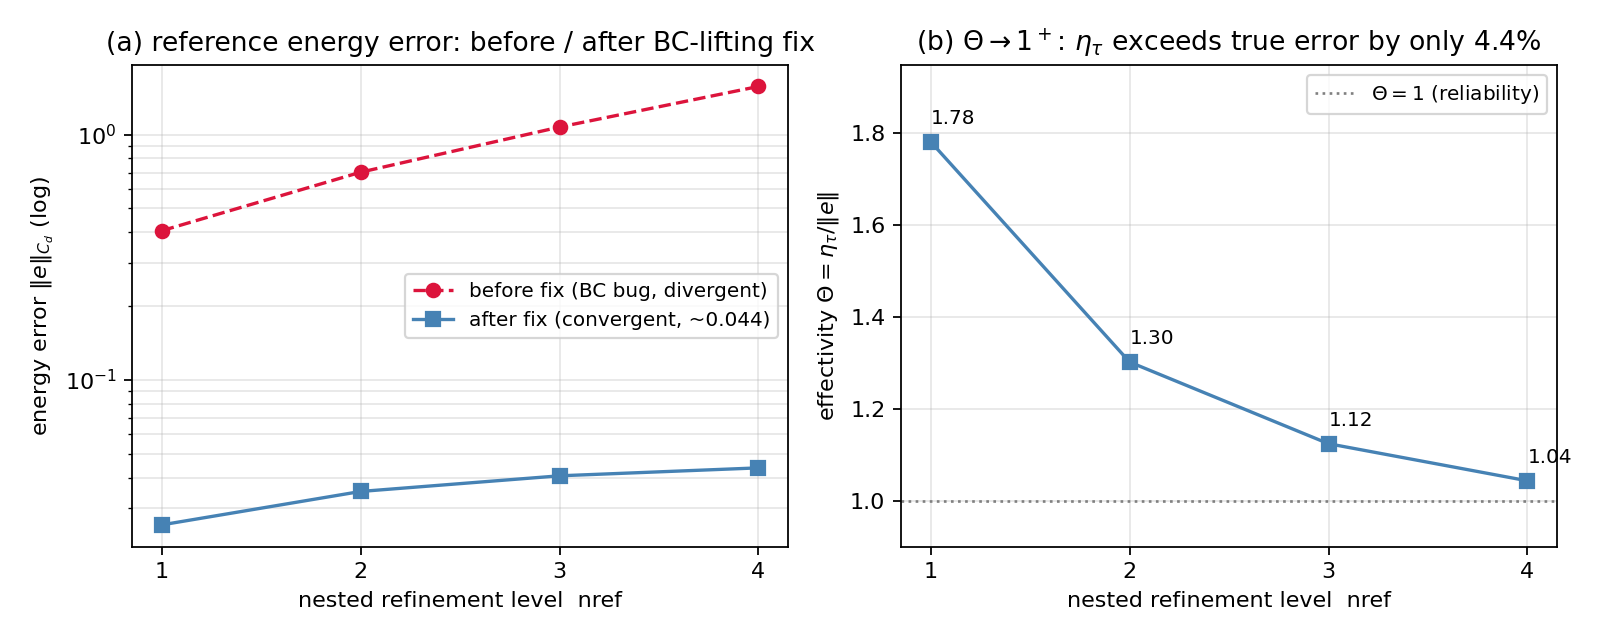
\includegraphics[width=\textwidth]{adaptive_theta_convergence.png}
\caption{Left: energy error of the reference solution versus nested refinement
level (a faithful conforming re-solve converges; an inconsistent Dirichlet
lifting would diverge). Right: effectivity index $\Theta=\eta/\|e\|\to1^+$,
exceeding the true error by $4.4\%$.}
\label{fig:theta}
\end{figure}

\paragraph{Equal-accuracy efficiency.}
Taking the peak reaction as the physical accuracy criterion (reference: a fine
uniform mesh, $476{,}883$ stress DOF), coarse uniform meshes overestimate the
peak by $+25\%$ to $+37\%$ (the under-resolution effect), whereas adaptivity
attains $-1.5\%$ using only $31{,}406$ stress DOF -- a $93\%$ reduction at
matched peak accuracy (Figure~\ref{fig:eff}). This quantifies why adaptivity is
necessary rather than merely economical: a coarse uniform mesh cannot recover
the correct peak at all.
\begin{figure}[t]\centering
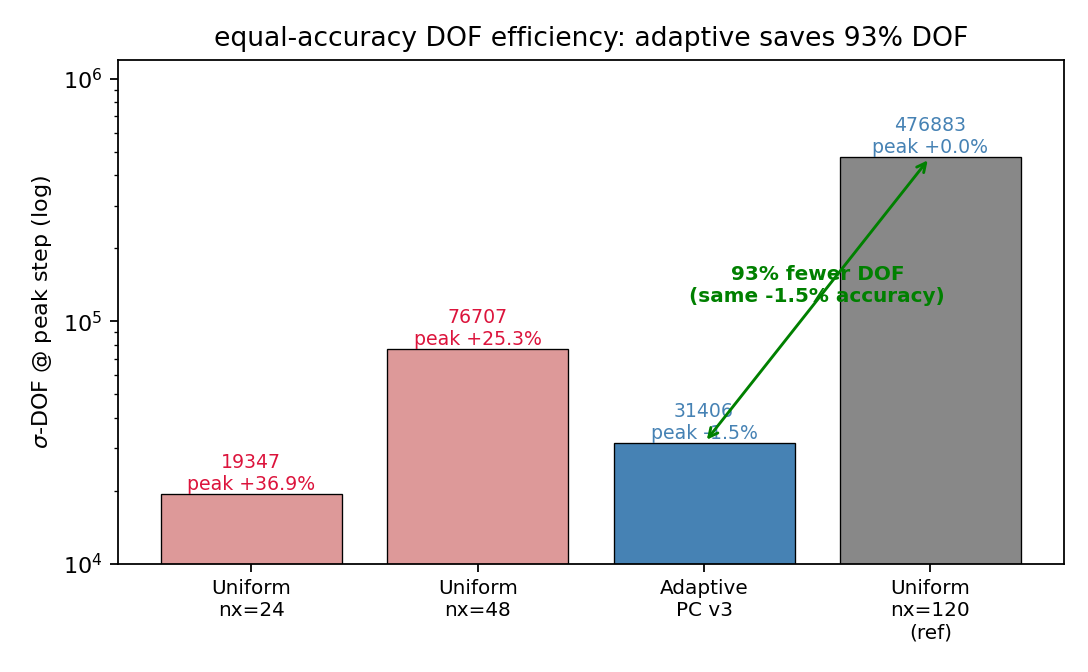
\includegraphics[width=0.62\textwidth]{adaptive_efficiency_dof.png}
\caption{Equal-accuracy stress-DOF comparison. Adaptive attains the reference
peak ($-1.5\%$) with $93\%$ fewer DOF; coarse uniform meshes are far off
($+25\%/+37\%$).}
\label{fig:eff}
\end{figure}

\paragraph{Single-edge shear.}
% TODO(model2): 后台 run results/adaptive_m3_pc_model2 完成后填入
% 峰值反力 / σ-DOF@peak / 失效曲线，并加载荷--位移图。
A single-edge shear specimen is reported to confirm the method on a second
loading mode; results are summarized in Table~\ref{tab:summary}
\emph{[pending background run]}.

\begin{table}[t]\centering
\caption{Summary across specimens (peak reaction vs.\ uniform reference;
stress DOF at peak step).}\label{tab:summary}
\begin{tabular}{lccc}
\toprule
specimen & peak dev.\ (\%) & $\sigma$-DOF @ peak & $\Theta$ (finest) \\
\midrule
edge tension (model 1) & $-1.5$ & $31{,}406$ & $1.044$ \\
edge shear (model 2)   & \emph{pending} & \emph{pending} & \emph{pending} \\
\bottomrule
\end{tabular}
\end{table}

\section{Conclusion}
A symmetric $H(\dv)$-conforming mixed stress turns the guaranteed equilibrated
estimator from a reconstruction problem into a direct one: reliability constant
one, no data oscillation in the canonical benchmark, and an effectivity that
follows the local (not global) coefficient contrast. The same stress drives a
predictive adaptive marking. Numerically, $\Theta\to1^+$ and adaptivity attains
matched peak accuracy with $93\%$ fewer degrees of freedom. Extensions: spectral
split majorant (dual potential), and certified marking beyond the predictor
loop.

\end{document}
